\documentclass[12pt, twoside,a4paper]{article}
\oddsidemargin = 10pt
\textwidth = 430pt

\usepackage{fullpage}	 %to make smaller margins
\usepackage{graphicx}
%\usepackage[utf8]{inputenc}
%\usepackage[T1]{fontenc}
%\usepackage{url}
\usepackage{hyperref}
\usepackage{pdfpages}
\usepackage{placeins}
\usepackage{graphicx}
\usepackage{caption}
\usepackage{subfig}

%\usepackage{subcaption}
\usepackage{enumerate}
\usepackage{amsmath}
\usepackage{listings} %for showing program code
\usepackage{bm}
\usepackage{wrapfig}
\usepackage{lipsum}
\usepackage{float}
\usepackage{titlesec}	
\usepackage{amsfonts}
\usepackage{amssymb}

\usepackage{epstopdf}

%\titlespacing*{\chapter}{0pt}{-10pt}{20pt}
%\titleformat{\chapter}[display]{\normalfont\huge\bfseries}{}{35pt}{}

\setlength{\intextsep}{0pt} %to make wrapfigures beautiful
%\setlength{\oddsidemargin}{0.5cm}
%\setlength{\evensidemargin}{-0.5cm}
\begin{document}

\title{Real-Time Rendering of Translucent Materials with Directional Subsurface Scattering}
\date{19 February 2014}
\author{Alessandro Dal Corso}
\maketitle
\section{Introduction (draft)}
\emph{Subsurface scattering} (SS) is a physical phenomenon that naturally occurs in a wide range of natural materials. Some of the materials that exhibit a strong SS effect in everyday life are milk, human skin and marble. Subsurface scattering is that phenomenon that occurs when light is partially absorbed by an object, bounces inside ("scatters") and finally exits the surface on another point of the material. The phenomenon that results is generally known as \emph{translucency}. We can see some examples of translucency in Figure \ref{fig:ex1}

Since the beginning of computer graphics, various attempts have been performed in order to physically model subsurface scattering. Some of these models involve physical simulations of the light entering the medium, other focus on approximating the diffusion of light within the material using an analytical approach.
 

The first model that did not involved a physical simulation was proposed by Jensen, as an approximation of the radiative diffusion equation. A radiative diffusion equation analytical approximation has then been exploited by different authors, in order to account for multi-layered materials, highly absorbing materials and thin surfaces. A recent analytical approximation, proposed by Frisvad, extends the approximation in order to account for the directionality of the incoming light. 


In recent years, with the advent of programmable graphics cards (GPU), it has become possible to exploit these algorithms and bring them to interactive frame rates, and in some cases even to real time rendering. Jensen and Buhler were the first to propose an interactive technique for rendering subsurface scattering using an octree. More recently, several methods have been proposed, including image-based splats, sum-of-Gaussians filtering, and grid-propagation based methods.

In this thesis we want to employ some cutting edge GPU techniques, with the aid of the programmable pipeline, to implement Frisvad directional model in a real-time fashion. This method should achieve real time results (i.e. in the range of 30 to 60 frames per second) for a wide range of natural materials.

\begin{figure}
\centering
\subfloat{
  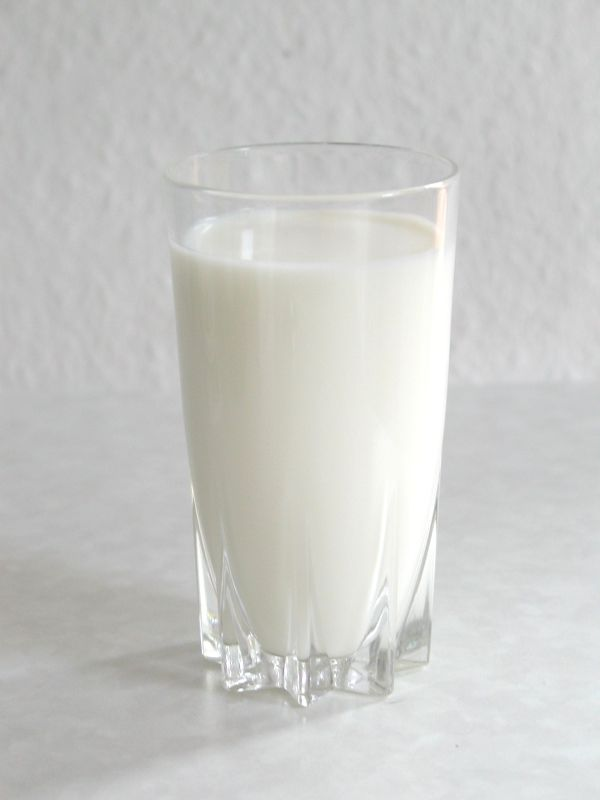
\includegraphics[width=0.3 \linewidth]{images/milk}
  \label{fig:or}
}
\subfloat{
  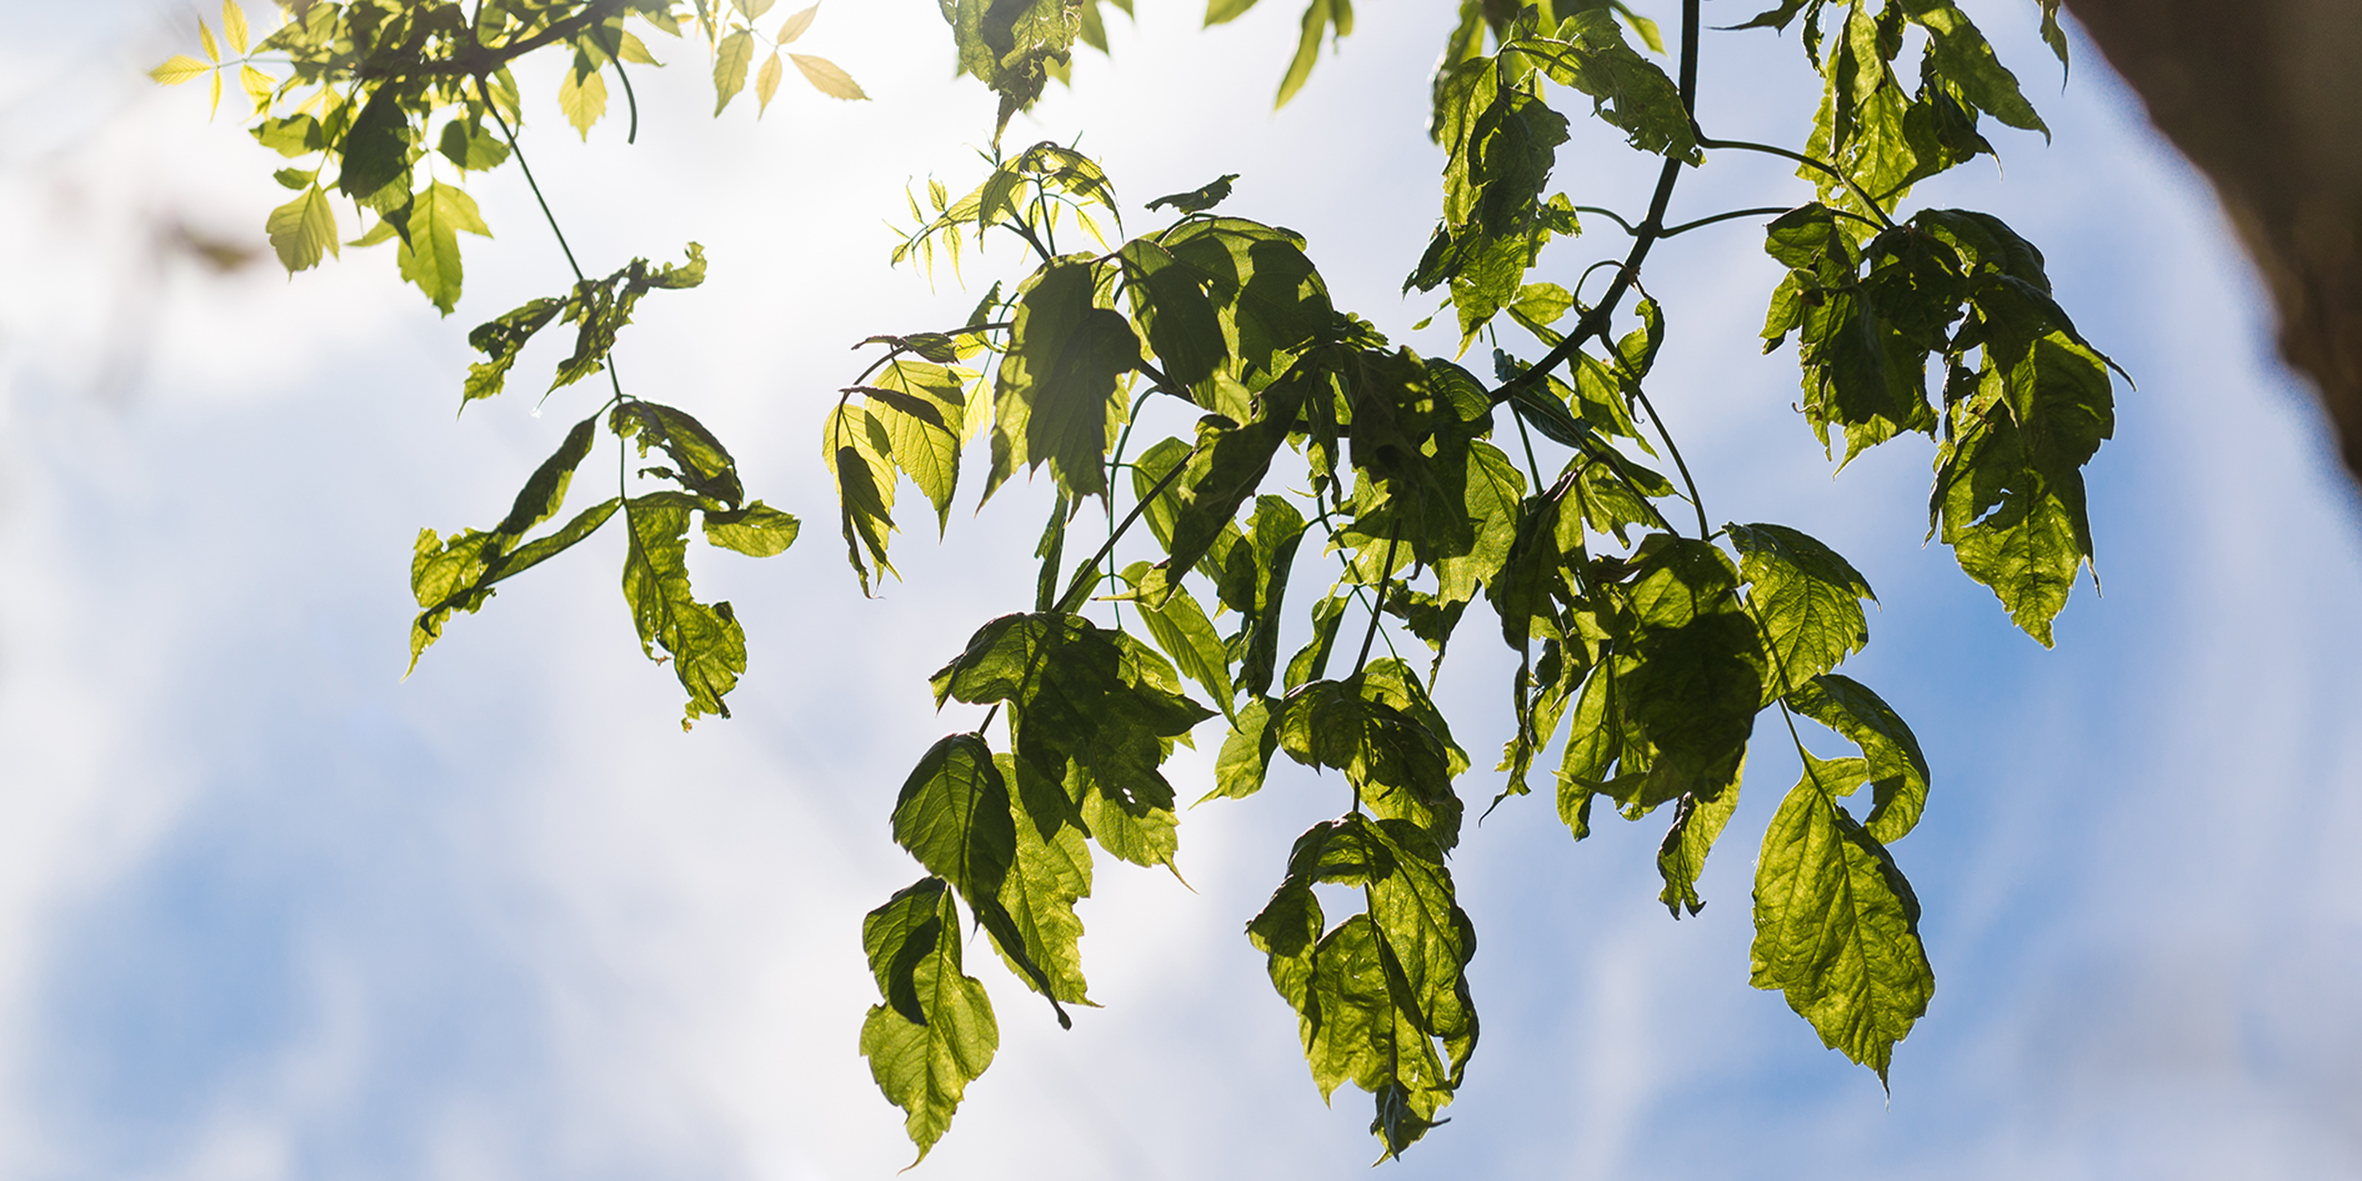
\includegraphics[width=0.3 \linewidth]{images/leaves}
  \label{fig:ex}
} 
\caption{Some examples of translucent materials: milk and leaves.}
\label{fig:ex1}
\end{figure}
\FloatBarrier

\end{document}
